\PassOptionsToPackage{unicode=true}{hyperref} % options for packages loaded elsewhere
\PassOptionsToPackage{hyphens}{url}
%
\documentclass[]{article}
\usepackage{lmodern}
\usepackage{amssymb,amsmath}
\usepackage{ifxetex,ifluatex}
\usepackage{fixltx2e} % provides \textsubscript
\ifnum 0\ifxetex 1\fi\ifluatex 1\fi=0 % if pdftex
  \usepackage[T1]{fontenc}
  \usepackage[utf8]{inputenc}
  \usepackage{textcomp} % provides euro and other symbols
\else % if luatex or xelatex
  \usepackage{unicode-math}
  \defaultfontfeatures{Ligatures=TeX,Scale=MatchLowercase}
\fi
% use upquote if available, for straight quotes in verbatim environments
\IfFileExists{upquote.sty}{\usepackage{upquote}}{}
% use microtype if available
\IfFileExists{microtype.sty}{%
\usepackage[]{microtype}
\UseMicrotypeSet[protrusion]{basicmath} % disable protrusion for tt fonts
}{}
\IfFileExists{parskip.sty}{%
\usepackage{parskip}
}{% else
\setlength{\parindent}{0pt}
\setlength{\parskip}{6pt plus 2pt minus 1pt}
}
\usepackage{hyperref}
\hypersetup{
            pdftitle={Processing Text Data},
            pdfauthor={Jeff Cavanagh},
            pdfborder={0 0 0},
            breaklinks=true}
\urlstyle{same}  % don't use monospace font for urls
\usepackage[margin=1in]{geometry}
\usepackage{color}
\usepackage{fancyvrb}
\newcommand{\VerbBar}{|}
\newcommand{\VERB}{\Verb[commandchars=\\\{\}]}
\DefineVerbatimEnvironment{Highlighting}{Verbatim}{commandchars=\\\{\}}
% Add ',fontsize=\small' for more characters per line
\usepackage{framed}
\definecolor{shadecolor}{RGB}{248,248,248}
\newenvironment{Shaded}{\begin{snugshade}}{\end{snugshade}}
\newcommand{\AlertTok}[1]{\textcolor[rgb]{0.94,0.16,0.16}{#1}}
\newcommand{\AnnotationTok}[1]{\textcolor[rgb]{0.56,0.35,0.01}{\textbf{\textit{#1}}}}
\newcommand{\AttributeTok}[1]{\textcolor[rgb]{0.77,0.63,0.00}{#1}}
\newcommand{\BaseNTok}[1]{\textcolor[rgb]{0.00,0.00,0.81}{#1}}
\newcommand{\BuiltInTok}[1]{#1}
\newcommand{\CharTok}[1]{\textcolor[rgb]{0.31,0.60,0.02}{#1}}
\newcommand{\CommentTok}[1]{\textcolor[rgb]{0.56,0.35,0.01}{\textit{#1}}}
\newcommand{\CommentVarTok}[1]{\textcolor[rgb]{0.56,0.35,0.01}{\textbf{\textit{#1}}}}
\newcommand{\ConstantTok}[1]{\textcolor[rgb]{0.00,0.00,0.00}{#1}}
\newcommand{\ControlFlowTok}[1]{\textcolor[rgb]{0.13,0.29,0.53}{\textbf{#1}}}
\newcommand{\DataTypeTok}[1]{\textcolor[rgb]{0.13,0.29,0.53}{#1}}
\newcommand{\DecValTok}[1]{\textcolor[rgb]{0.00,0.00,0.81}{#1}}
\newcommand{\DocumentationTok}[1]{\textcolor[rgb]{0.56,0.35,0.01}{\textbf{\textit{#1}}}}
\newcommand{\ErrorTok}[1]{\textcolor[rgb]{0.64,0.00,0.00}{\textbf{#1}}}
\newcommand{\ExtensionTok}[1]{#1}
\newcommand{\FloatTok}[1]{\textcolor[rgb]{0.00,0.00,0.81}{#1}}
\newcommand{\FunctionTok}[1]{\textcolor[rgb]{0.00,0.00,0.00}{#1}}
\newcommand{\ImportTok}[1]{#1}
\newcommand{\InformationTok}[1]{\textcolor[rgb]{0.56,0.35,0.01}{\textbf{\textit{#1}}}}
\newcommand{\KeywordTok}[1]{\textcolor[rgb]{0.13,0.29,0.53}{\textbf{#1}}}
\newcommand{\NormalTok}[1]{#1}
\newcommand{\OperatorTok}[1]{\textcolor[rgb]{0.81,0.36,0.00}{\textbf{#1}}}
\newcommand{\OtherTok}[1]{\textcolor[rgb]{0.56,0.35,0.01}{#1}}
\newcommand{\PreprocessorTok}[1]{\textcolor[rgb]{0.56,0.35,0.01}{\textit{#1}}}
\newcommand{\RegionMarkerTok}[1]{#1}
\newcommand{\SpecialCharTok}[1]{\textcolor[rgb]{0.00,0.00,0.00}{#1}}
\newcommand{\SpecialStringTok}[1]{\textcolor[rgb]{0.31,0.60,0.02}{#1}}
\newcommand{\StringTok}[1]{\textcolor[rgb]{0.31,0.60,0.02}{#1}}
\newcommand{\VariableTok}[1]{\textcolor[rgb]{0.00,0.00,0.00}{#1}}
\newcommand{\VerbatimStringTok}[1]{\textcolor[rgb]{0.31,0.60,0.02}{#1}}
\newcommand{\WarningTok}[1]{\textcolor[rgb]{0.56,0.35,0.01}{\textbf{\textit{#1}}}}
\usepackage{graphicx,grffile}
\makeatletter
\def\maxwidth{\ifdim\Gin@nat@width>\linewidth\linewidth\else\Gin@nat@width\fi}
\def\maxheight{\ifdim\Gin@nat@height>\textheight\textheight\else\Gin@nat@height\fi}
\makeatother
% Scale images if necessary, so that they will not overflow the page
% margins by default, and it is still possible to overwrite the defaults
% using explicit options in \includegraphics[width, height, ...]{}
\setkeys{Gin}{width=\maxwidth,height=\maxheight,keepaspectratio}
\setlength{\emergencystretch}{3em}  % prevent overfull lines
\providecommand{\tightlist}{%
  \setlength{\itemsep}{0pt}\setlength{\parskip}{0pt}}
\setcounter{secnumdepth}{0}
% Redefines (sub)paragraphs to behave more like sections
\ifx\paragraph\undefined\else
\let\oldparagraph\paragraph
\renewcommand{\paragraph}[1]{\oldparagraph{#1}\mbox{}}
\fi
\ifx\subparagraph\undefined\else
\let\oldsubparagraph\subparagraph
\renewcommand{\subparagraph}[1]{\oldsubparagraph{#1}\mbox{}}
\fi

% set default figure placement to htbp
\makeatletter
\def\fps@figure{htbp}
\makeatother


\title{Processing Text Data}
\author{Jeff Cavanagh}
\date{2020-08-05}

\begin{document}
\maketitle

\textbf{Text data cannot be processed identically to numerical or
categorical data. Is there a way then to analyze text data insight from
it??}

Of course! All it takes is an adapted approach and a little more work
upfront.

Quite a bit of potential data is unstructured and textual in nature, and
does not operate by the same rules as numerical or categorical data.
That does not mean there is not value to this format of data though. To
extract that value, different techniques are required.

In this post we will focus on some routine methods for text mining and
text analysis in R and how they can be utilized to process and draw
value from text data.

\hypertarget{setup}{%
\subsection{Setup}\label{setup}}

\hypertarget{stringr}{%
\subsubsection{\texorpdfstring{\texttt{stringr}}{stringr}}\label{stringr}}

In R, the best way I have found to carry out any sort of NLP is using
the \texttt{stringr} package. This package can be loaded on its own, or
as part of \texttt{tidyverse}.

The functions contained with in all process character strings in various
ways. Luckily for us, R has a
\href{/rcheatsheets/strings.pdf}{cheatsheet} for the \texttt{stringr}
package for not only the functions, but also the formatting of search
patterns.

It should be noted that there is also the \texttt{stringi} package which
contains more robust functions for handling strings. For simplicity, we
will only be concentrating on \texttt{stringr} so let's load that now.

\begin{Shaded}
\begin{Highlighting}[]
\KeywordTok{library}\NormalTok{(stringr)}
\KeywordTok{library}\NormalTok{(tidyverse)}
\end{Highlighting}
\end{Shaded}

\hypertarget{the-data}{%
\subsubsection{The Data}\label{the-data}}

To illustrate the use of NLP, we will be analyzing a pdf of Mary
Shelley's, \emph{Frankenstein} (downloaded from
\href{https://www.planetebook.com/free-ebooks/frankenstein.pdf}{planetbook.com}).
We will use the \texttt{pdftools} package to extract the text from the
pdf file.

\begin{Shaded}
\begin{Highlighting}[]
\KeywordTok{library}\NormalTok{(pdftools)}
\NormalTok{book <-}\StringTok{ }\KeywordTok{pdf_text}\NormalTok{(}\StringTok{"frankenstein.pdf"}\NormalTok{)}
\end{Highlighting}
\end{Shaded}

\texttt{pdf\_text} from the \texttt{pdf\_tools} package converts the pdf
file into a character string where each element is a page from the
document.

Now that we have the defined the book as a character string we will
begin to mold it into a dataframe so it is easier to work with.

\begin{Shaded}
\begin{Highlighting}[]
\NormalTok{book_df <-}\StringTok{ }\NormalTok{book  }\OperatorTok\StringTok{ }
\StringTok{  }\KeywordTok{as_tibble_col}\NormalTok{(}\StringTok{"content"}\NormalTok{) }\OperatorTok
\StringTok{  }\KeywordTok{rowid_to_column}\NormalTok{(}\StringTok{"page_number"}\NormalTok{)}

\NormalTok{book_df}
\end{Highlighting}
\end{Shaded}

\begin{verbatim}
## # A tibble: 277 x 2
##    page_number content                                                          
##          <int> <chr>                                                            
##  1           1 "Frankenstein\nBy Mary Wollstonecraft Shelley\nDownload free eBo~
##  2           2 "Letter 1\nTo Mrs. Saville, England\n   St. Petersburgh, Dec. 11~
##  3           3 "and features may be without example, as the phenomena of\nthe h~
##  4           4 "North Pacific Ocean through the seas which surround the\npole. ~
##  5           5 "practical advantage. Twice I actually hired myself as an un-\nd~
##  6           6 "easily be done by paying the insurance for the owner, and\nto e~
##  7           7 "Letter 2\nTo Mrs. Saville, England\n   Archangel, 28th March, 1~
##  8           8 "to me that I am self-educated: for the first fourteen years\nof~
##  9           9 "remarkable in the ship for his gentleness and the mildness of\n~
## 10          10 "himself bound in honour to my friend, who, when he found\nthe f~
## # ... with 267 more rows
\end{verbatim}

We know have a data frame, where each row is an observation containing
the page number and content held on that page. Now let's look for
patterns.

\begin{itemize}
\tightlist
\item
  \texttt{str\_detect} can be used to detect which observations match a
  pattern
\item
  \texttt{str\_which} can be used to pick out the index's of the entries
  of all matches
\item
  \texttt{str\_extract} can be used to pull out the first pattern match
  within each element

  \begin{itemize}
  \tightlist
  \item
    Some functions in \texttt{stringr} also have a \texttt{\_all}
    functionality, such as \texttt{str\_extract\_all}, which returns all
    matches within an observation
  \end{itemize}
\end{itemize}

Here is a look at how these three function in practice. To illustrate
the use of these functions, we will search for all pages that reference
``Frankenstein''.

(\texttt{\^{}} is used to search for matches at the start of a string,
\texttt{.} is used to match any character that is not a new line,
\texttt{{[}:upper:{]}} is used to match upper case words, and \texttt{*}
is used to pull 0 or more matches).

\begin{Shaded}
\begin{Highlighting}[]
\NormalTok{book_df}\OperatorTok{$}\NormalTok{content }\OperatorTok
\StringTok{  }\KeywordTok{str_detect}\NormalTok{(}\StringTok{"Frankenstein"}\NormalTok{)}
\end{Highlighting}
\end{Shaded}

\begin{verbatim}
##   [1]  TRUE  TRUE FALSE  TRUE FALSE  TRUE FALSE  TRUE FALSE  TRUE FALSE  TRUE
##  [13] FALSE  TRUE FALSE  TRUE FALSE  TRUE FALSE  TRUE FALSE  TRUE FALSE  TRUE
##  [25] FALSE  TRUE FALSE  TRUE FALSE  TRUE FALSE  TRUE FALSE  TRUE FALSE  TRUE
##  [37] FALSE  TRUE FALSE  TRUE FALSE  TRUE FALSE  TRUE FALSE  TRUE FALSE  TRUE
##  [49] FALSE  TRUE FALSE  TRUE FALSE  TRUE FALSE  TRUE FALSE  TRUE FALSE  TRUE
##  [61]  TRUE  TRUE FALSE  TRUE FALSE  TRUE FALSE  TRUE FALSE  TRUE FALSE  TRUE
##  [73]  TRUE  TRUE FALSE  TRUE FALSE  TRUE  TRUE  TRUE FALSE  TRUE FALSE  TRUE
##  [85] FALSE  TRUE FALSE  TRUE FALSE  TRUE FALSE  TRUE FALSE  TRUE FALSE  TRUE
##  [97] FALSE  TRUE FALSE  TRUE FALSE  TRUE FALSE  TRUE FALSE  TRUE FALSE  TRUE
## [109] FALSE  TRUE FALSE  TRUE FALSE  TRUE  TRUE  TRUE FALSE  TRUE FALSE  TRUE
## [121] FALSE  TRUE FALSE  TRUE FALSE  TRUE FALSE  TRUE FALSE  TRUE FALSE  TRUE
## [133] FALSE  TRUE FALSE  TRUE FALSE  TRUE FALSE  TRUE FALSE  TRUE FALSE  TRUE
## [145] FALSE  TRUE FALSE  TRUE FALSE  TRUE FALSE  TRUE FALSE  TRUE FALSE  TRUE
## [157] FALSE  TRUE FALSE  TRUE FALSE  TRUE FALSE  TRUE FALSE  TRUE FALSE  TRUE
## [169] FALSE  TRUE  TRUE  TRUE FALSE  TRUE FALSE  TRUE FALSE  TRUE FALSE  TRUE
## [181] FALSE  TRUE FALSE  TRUE FALSE  TRUE FALSE  TRUE FALSE  TRUE FALSE  TRUE
## [193] FALSE  TRUE FALSE  TRUE FALSE  TRUE FALSE  TRUE FALSE  TRUE FALSE  TRUE
## [205] FALSE  TRUE FALSE  TRUE FALSE  TRUE FALSE  TRUE FALSE  TRUE FALSE  TRUE
## [217] FALSE  TRUE FALSE  TRUE FALSE  TRUE FALSE  TRUE FALSE  TRUE FALSE  TRUE
## [229] FALSE  TRUE FALSE  TRUE FALSE  TRUE FALSE  TRUE FALSE  TRUE FALSE  TRUE
## [241] FALSE  TRUE FALSE  TRUE FALSE  TRUE FALSE  TRUE FALSE  TRUE FALSE  TRUE
## [253] FALSE  TRUE FALSE  TRUE FALSE  TRUE FALSE  TRUE FALSE  TRUE FALSE  TRUE
## [265]  TRUE  TRUE FALSE  TRUE FALSE  TRUE  TRUE  TRUE  TRUE  TRUE FALSE  TRUE
## [277] FALSE
\end{verbatim}

\begin{Shaded}
\begin{Highlighting}[]
\NormalTok{book_df}\OperatorTok{$}\NormalTok{content }\OperatorTok
\StringTok{  }\KeywordTok{str_detect}\NormalTok{(}\StringTok{"Frankenstein"}\NormalTok{) }\OperatorTok
\StringTok{  }\KeywordTok{sum}\NormalTok{()}
\end{Highlighting}
\end{Shaded}

\begin{verbatim}
## [1] 147
\end{verbatim}

\begin{Shaded}
\begin{Highlighting}[]
\NormalTok{book_df}\OperatorTok{$}\NormalTok{content }\OperatorTok
\StringTok{  }\KeywordTok{str_detect}\NormalTok{(}\StringTok{"Frankenstein"}\NormalTok{) }\OperatorTok
\StringTok{  }\KeywordTok{mean}\NormalTok{()}
\end{Highlighting}
\end{Shaded}

\begin{verbatim}
## [1] 0.5306859
\end{verbatim}

Adding on the \texttt{sum} and \texttt{mean} functions we are also able
to see the number and percentage of pages which contain the
``Frankenstein'' text pattern.

Next, \texttt{str\_which} gives us the locations of the pages containing
the pattern.

\begin{Shaded}
\begin{Highlighting}[]
\NormalTok{ind_capitals <-}\StringTok{ }\NormalTok{book_df}\OperatorTok{$}\NormalTok{content }\OperatorTok
\StringTok{  }\KeywordTok{str_which}\NormalTok{(}\StringTok{"Frankenstein"}\NormalTok{)}

\NormalTok{ind_capitals}
\end{Highlighting}
\end{Shaded}

\begin{verbatim}
##   [1]   1   2   4   6   8  10  12  14  16  18  20  22  24  26  28  30  32  34
##  [19]  36  38  40  42  44  46  48  50  52  54  56  58  60  61  62  64  66  68
##  [37]  70  72  73  74  76  78  79  80  82  84  86  88  90  92  94  96  98 100
##  [55] 102 104 106 108 110 112 114 115 116 118 120 122 124 126 128 130 132 134
##  [73] 136 138 140 142 144 146 148 150 152 154 156 158 160 162 164 166 168 170
##  [91] 171 172 174 176 178 180 182 184 186 188 190 192 194 196 198 200 202 204
## [109] 206 208 210 212 214 216 218 220 222 224 226 228 230 232 234 236 238 240
## [127] 242 244 246 248 250 252 254 256 258 260 262 264 265 266 268 270 271 272
## [145] 273 274 276
\end{verbatim}

Lastly, \texttt{str\_extract} pulls the pattern from each of the pages.
However, \texttt{str\_extract} will return a vector as the same length
as the input. In order to filter to only entries that have the pattern
match, we will combine it with \texttt{str\_which}.

\begin{Shaded}
\begin{Highlighting}[]
\NormalTok{book_df}\OperatorTok{$}\NormalTok{content[ind_capitals] }\OperatorTok
\StringTok{  }\KeywordTok{str_extract}\NormalTok{(}\StringTok{"Frankenstein"}\NormalTok{)}
\end{Highlighting}
\end{Shaded}

\begin{verbatim}
##   [1] "Frankenstein" "Frankenstein" "Frankenstein" "Frankenstein" "Frankenstein"
##   [6] "Frankenstein" "Frankenstein" "Frankenstein" "Frankenstein" "Frankenstein"
##  [11] "Frankenstein" "Frankenstein" "Frankenstein" "Frankenstein" "Frankenstein"
##  [16] "Frankenstein" "Frankenstein" "Frankenstein" "Frankenstein" "Frankenstein"
##  [21] "Frankenstein" "Frankenstein" "Frankenstein" "Frankenstein" "Frankenstein"
##  [26] "Frankenstein" "Frankenstein" "Frankenstein" "Frankenstein" "Frankenstein"
##  [31] "Frankenstein" "Frankenstein" "Frankenstein" "Frankenstein" "Frankenstein"
##  [36] "Frankenstein" "Frankenstein" "Frankenstein" "Frankenstein" "Frankenstein"
##  [41] "Frankenstein" "Frankenstein" "Frankenstein" "Frankenstein" "Frankenstein"
##  [46] "Frankenstein" "Frankenstein" "Frankenstein" "Frankenstein" "Frankenstein"
##  [51] "Frankenstein" "Frankenstein" "Frankenstein" "Frankenstein" "Frankenstein"
##  [56] "Frankenstein" "Frankenstein" "Frankenstein" "Frankenstein" "Frankenstein"
##  [61] "Frankenstein" "Frankenstein" "Frankenstein" "Frankenstein" "Frankenstein"
##  [66] "Frankenstein" "Frankenstein" "Frankenstein" "Frankenstein" "Frankenstein"
##  [71] "Frankenstein" "Frankenstein" "Frankenstein" "Frankenstein" "Frankenstein"
##  [76] "Frankenstein" "Frankenstein" "Frankenstein" "Frankenstein" "Frankenstein"
##  [81] "Frankenstein" "Frankenstein" "Frankenstein" "Frankenstein" "Frankenstein"
##  [86] "Frankenstein" "Frankenstein" "Frankenstein" "Frankenstein" "Frankenstein"
##  [91] "Frankenstein" "Frankenstein" "Frankenstein" "Frankenstein" "Frankenstein"
##  [96] "Frankenstein" "Frankenstein" "Frankenstein" "Frankenstein" "Frankenstein"
## [101] "Frankenstein" "Frankenstein" "Frankenstein" "Frankenstein" "Frankenstein"
## [106] "Frankenstein" "Frankenstein" "Frankenstein" "Frankenstein" "Frankenstein"
## [111] "Frankenstein" "Frankenstein" "Frankenstein" "Frankenstein" "Frankenstein"
## [116] "Frankenstein" "Frankenstein" "Frankenstein" "Frankenstein" "Frankenstein"
## [121] "Frankenstein" "Frankenstein" "Frankenstein" "Frankenstein" "Frankenstein"
## [126] "Frankenstein" "Frankenstein" "Frankenstein" "Frankenstein" "Frankenstein"
## [131] "Frankenstein" "Frankenstein" "Frankenstein" "Frankenstein" "Frankenstein"
## [136] "Frankenstein" "Frankenstein" "Frankenstein" "Frankenstein" "Frankenstein"
## [141] "Frankenstein" "Frankenstein" "Frankenstein" "Frankenstein" "Frankenstein"
## [146] "Frankenstein" "Frankenstein"
\end{verbatim}

\hypertarget{cleaning-the-data}{%
\subsubsection{Cleaning the Data}\label{cleaning-the-data}}

The text data in now in a dataframe, but is still far from orderly.
Perusing through a few pages reveals that the footer at the bottom of
each page is either the page number (which we already have) and the
title of the book (Frankenstein), or the page number and the website
home of the pdf.

Neither of these are useful to us. Let's use \texttt{str\_remove} to
remove these from the pages.

\begin{Shaded}
\begin{Highlighting}[]
\NormalTok{book_df}\OperatorTok{$}\NormalTok{content <-}\StringTok{ }\NormalTok{book_df}\OperatorTok{$}\NormalTok{content }\OperatorTok
\StringTok{  }\KeywordTok{str_remove}\NormalTok{(}\StringTok{"}\CharTok{\textbackslash{}\textbackslash{}}\StringTok{n(}\CharTok{\textbackslash{}\textbackslash{}}\StringTok{d+|}\CharTok{\textbackslash{}\textbackslash{}}\StringTok{030)}\CharTok{\textbackslash{}\textbackslash{}}\StringTok{s+Frankenstein}\CharTok{\textbackslash{}n}\StringTok{$|}\CharTok{\textbackslash{}\textbackslash{}}\StringTok{nFree eBooks at Planet eBook.com}\CharTok{\textbackslash{}\textbackslash{}}\StringTok{s+(}\CharTok{\textbackslash{}\textbackslash{}}\StringTok{d+|}\CharTok{\textbackslash{}\textbackslash{}\textbackslash{}030}\StringTok{)}\CharTok{\textbackslash{}\textbackslash{}}\StringTok{n$"}\NormalTok{)}
\end{Highlighting}
\end{Shaded}

\begin{itemize}
\tightlist
\item
  \texttt{\$} is used to search for the pattern at the end of each
  string
\item
  \texttt{\textbackslash{}\textbackslash{}n} is used to detect new lines
\item
  \texttt{\textbackslash{}\textbackslash{}d} is used to detect digits
\item
  \texttt{\textbackslash{}\textbackslash{}s} is used to detect and
  spaces
\item
  \texttt{\textbackslash{}\textbackslash{}\textbackslash{}} is used to
  detect a back slash
\item
  \texttt{+} is used to detect 1 or more occurences of the character
  that comes immediately before
\item
  \texttt{\textbar{}} is used as an or statement to detect multiple
  patterns
\end{itemize}

\hypertarget{breaking-down-text-data}{%
\subsubsection{Breaking Down Text Data}\label{breaking-down-text-data}}

Now our strings contain only the most relevant information, but they are
still dense and difficult to decipher insight from.

The next step is to use the \texttt{tidytext} package to further break
up the data. Using the \texttt{unnest\_token} function it is possible to
breakdown character strings into lines, paragraphs, sentences, words,
and n-grams. First we will update the data frame by breaking the strings
down by line.

\begin{Shaded}
\begin{Highlighting}[]
\KeywordTok{library}\NormalTok{(tidytext)}

\NormalTok{book_df <-}\StringTok{ }\NormalTok{book_df }\OperatorTok
\StringTok{  }\KeywordTok{unnest_tokens}\NormalTok{(}\StringTok{"lines"}\NormalTok{, content, }\DataTypeTok{token =} \StringTok{"lines"}\NormalTok{, }\DataTypeTok{to_lower =}\NormalTok{ F)}

\NormalTok{book_df}
\end{Highlighting}
\end{Shaded}

\begin{verbatim}
## # A tibble: 7,585 x 2
##    page_number lines                                                         
##          <int> <chr>                                                         
##  1           1 "Frankenstein"                                                
##  2           1 "By Mary Wollstonecraft Shelley"                              
##  3           1 "Download free eBooks of classic literature, books and"       
##  4           1 "novels at Planet eBook. Subscribe to our free eBooks blog"   
##  5           1 "and email newsletter."                                       
##  6           2 "Letter 1"                                                    
##  7           2 "To Mrs. Saville, England"                                    
##  8           2 "   St. Petersburgh, Dec. 11th, 17—"                          
##  9           2 "   You will rejoice to hear that no disaster has accompanied"
## 10           2 "the commencement of an enterprise which you have regard-"    
## # ... with 7,575 more rows
\end{verbatim}

Now that we have the text broken up into lines it is much easier to
process. Next lets add more identifying variables where each line can be
indentified by linenumber and the chapter.

\emph{Frankenstein} begins with several letters before it gets into the
chapters. To identify which pages fall under letters or chapters, and
what numbers within, we need to do a little preliminary work with the
tools demonstrated so far.

\begin{Shaded}
\begin{Highlighting}[]
\NormalTok{ind_chapter <-}\StringTok{ }\NormalTok{book_df}\OperatorTok{$}\NormalTok{lines }\OperatorTok
\StringTok{  }\KeywordTok{str_which}\NormalTok{(}\StringTok{"^Chapter"}\NormalTok{) }\OperatorTok
\StringTok{  }\KeywordTok{append}\NormalTok{(}\KeywordTok{nrow}\NormalTok{(book_df))}

\NormalTok{chapters <-}\StringTok{ }\NormalTok{book_df}\OperatorTok{$}\NormalTok{lines[ind_chapter[}\OperatorTok{-}\KeywordTok{length}\NormalTok{(ind_chapter)]] }\OperatorTok
\StringTok{  }\KeywordTok{str_extract}\NormalTok{(}\StringTok{"^Chapter.*"}\NormalTok{) }\OperatorTok
\StringTok{  }\KeywordTok{unlist}\NormalTok{()}

\NormalTok{ind_letter <-}\StringTok{ }\NormalTok{book_df}\OperatorTok{$}\NormalTok{lines }\OperatorTok
\StringTok{  }\KeywordTok{str_which}\NormalTok{(}\StringTok{"^Letter"}\NormalTok{) }\OperatorTok
\StringTok{  }\KeywordTok{append}\NormalTok{(ind_chapter[}\DecValTok{1}\NormalTok{])}

\NormalTok{letters <-}\StringTok{ }\NormalTok{book_df}\OperatorTok{$}\NormalTok{lines[ind_letter[}\OperatorTok{-}\KeywordTok{length}\NormalTok{(ind_letter)]] }\OperatorTok
\StringTok{  }\KeywordTok{str_extract_all}\NormalTok{(}\StringTok{"^Letter.*"}\NormalTok{) }\OperatorTok
\StringTok{  }\KeywordTok{unlist}\NormalTok{()}
\end{Highlighting}
\end{Shaded}

\begin{itemize}
\tightlist
\item
  \texttt{\^{}} searches the start of a string for a pattern
\item
  \texttt{.} matches any character that is not a new line
\item
  \texttt{*} matches zero or more of the character preceding it
\end{itemize}

Now that we have our indexes and values we can create new columns to
further classify each observation.

\begin{Shaded}
\begin{Highlighting}[]
\NormalTok{book_df <-}\StringTok{ }\NormalTok{book_df }\OperatorTok
\StringTok{  }\KeywordTok{mutate}\NormalTok{(}
    \DataTypeTok{line_number =} \KeywordTok{row_number}\NormalTok{(),}
    \DataTypeTok{chapter =} \StringTok{"fill in"}
\NormalTok{  )}
\NormalTok{book_df}\OperatorTok{$}\NormalTok{chapter[}\KeywordTok{c}\NormalTok{(}\DecValTok{1}\OperatorTok{:}\NormalTok{(ind_letter[}\DecValTok{1}\NormalTok{] }\OperatorTok{-}\StringTok{ }\DecValTok{1}\NormalTok{))] <-}\StringTok{ "Preface"}

\ControlFlowTok{for}\NormalTok{ (i }\ControlFlowTok{in} \DecValTok{1}\OperatorTok{:}\NormalTok{(}\KeywordTok{length}\NormalTok{(ind_letter) }\OperatorTok{-}\StringTok{ }\DecValTok{1}\NormalTok{))\{}
\NormalTok{  book_df}\OperatorTok{$}\NormalTok{chapter[}\KeywordTok{c}\NormalTok{(ind_letter[i]}\OperatorTok{:}\NormalTok{(ind_letter[i }\OperatorTok{+}\StringTok{ }\DecValTok{1}\NormalTok{] }\DecValTok{-1}\NormalTok{))] <-}\StringTok{ }\NormalTok{letters[i]}
\NormalTok{\}}

\ControlFlowTok{for}\NormalTok{ (i }\ControlFlowTok{in} \DecValTok{1}\OperatorTok{:}\NormalTok{(}\KeywordTok{length}\NormalTok{(ind_chapter) }\OperatorTok{-}\StringTok{ }\DecValTok{1}\NormalTok{))\{}
\NormalTok{  book_df}\OperatorTok{$}\NormalTok{chapter[}\KeywordTok{c}\NormalTok{(ind_chapter[i]}\OperatorTok{:}\NormalTok{(ind_chapter[i }\OperatorTok{+}\StringTok{ }\DecValTok{1}\NormalTok{] }\DecValTok{-1}\NormalTok{))] <-}\StringTok{ }\NormalTok{chapters[i]}
\NormalTok{\}}

\NormalTok{book_df <-}\StringTok{ }\NormalTok{book_df }\OperatorTok
\StringTok{  }\KeywordTok{select}\NormalTok{(chapter, page_number, line_number, lines)}
\end{Highlighting}
\end{Shaded}

\texttt{mutate} was used to add the new columns to the data frame and
then \texttt{for} loops were used to set the values of the
\emph{chapter} column using the indexes and values that were
established.

What was began as a pdf of unstructured text is now a structured data
frame with clear variables and observations. Going forward this will be
much easier to process and manipulate.

\hypertarget{word-analysis}{%
\subsubsection{Word Analysis}\label{word-analysis}}

Now that we have a structured data frame, lets look for the most common
words that appear within the text.

\begin{Shaded}
\begin{Highlighting}[]
\NormalTok{book_words <-}\StringTok{ }\NormalTok{book_df }\OperatorTok
\StringTok{  }\KeywordTok{unnest_tokens}\NormalTok{(word, lines, }\DataTypeTok{token =} \StringTok{"words"}\NormalTok{) }

\NormalTok{book_words }\OperatorTok
\StringTok{  }\KeywordTok{count}\NormalTok{(word, }\DataTypeTok{sort =}\NormalTok{ T)}
\end{Highlighting}
\end{Shaded}

\begin{verbatim}
## # A tibble: 7,903 x 2
##    word      n
##    <chr> <int>
##  1 the    4192
##  2 and    2977
##  3 i      2851
##  4 of     2649
##  5 to     2108
##  6 my     1780
##  7 a      1392
##  8 in     1155
##  9 was    1021
## 10 that   1017
## # ... with 7,893 more rows
\end{verbatim}

The most common words are unsuprisingly the filler words used found in
any text. To sort these words out we will use the \texttt{stop\_words}
dataframe, which is a list of these common words.

\begin{Shaded}
\begin{Highlighting}[]
\NormalTok{book_words <-}\StringTok{ }\NormalTok{book_words }\OperatorTok
\StringTok{  }\KeywordTok{anti_join}\NormalTok{(stop_words) }
\end{Highlighting}
\end{Shaded}

\begin{verbatim}
## Joining, by = "word"
\end{verbatim}

\begin{Shaded}
\begin{Highlighting}[]
\NormalTok{book_words }\OperatorTok
\StringTok{  }\KeywordTok{count}\NormalTok{(word, }\DataTypeTok{sort =}\NormalTok{ T)}
\end{Highlighting}
\end{Shaded}

\begin{verbatim}
## # A tibble: 7,404 x 2
##    word          n
##    <chr>     <int>
##  1 life        116
##  2 father      111
##  3 eyes        104
##  4 time         99
##  5 night        92
##  6 found        87
##  7 mind         84
##  8 day          82
##  9 elizabeth    82
## 10 heart        81
## # ... with 7,394 more rows
\end{verbatim}

Now that we have this count, it would be nice to have a visualization of
the most common words. Let's do that now using \texttt{ggplot}.

\begin{Shaded}
\begin{Highlighting}[]
\NormalTok{book_words }\OperatorTok
\StringTok{  }\KeywordTok{count}\NormalTok{(word, }\DataTypeTok{sort =}\NormalTok{ T) }\OperatorTok
\StringTok{  }\KeywordTok{filter}\NormalTok{(n }\OperatorTok{>}\StringTok{ }\DecValTok{60}\NormalTok{) }\OperatorTok
\StringTok{  }\KeywordTok{mutate}\NormalTok{(}\DataTypeTok{word =} \KeywordTok{reorder}\NormalTok{(word, n)) }\OperatorTok
\StringTok{  }\KeywordTok{ggplot}\NormalTok{() }\OperatorTok{+}
\StringTok{  }\KeywordTok{geom_col}\NormalTok{(}\KeywordTok{aes}\NormalTok{(n, word))}
\end{Highlighting}
\end{Shaded}

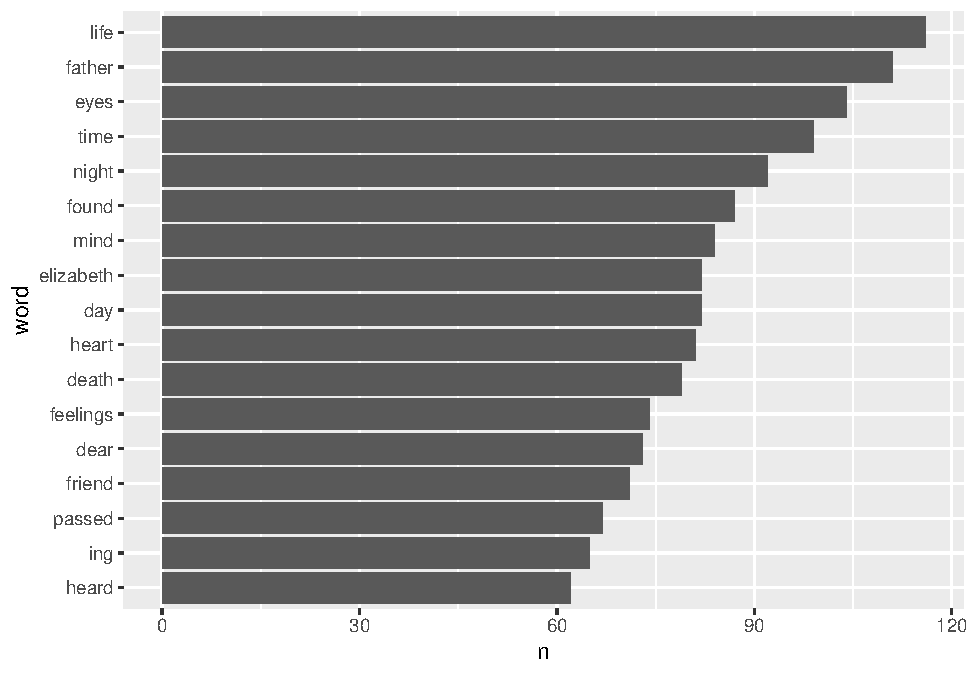
\includegraphics{2020-08-05-processing-text-data_files/figure-latex/unnamed-chunk-13-1.pdf}

\end{document}
